\documentclass{beamer}

\usepackage[utf8]{inputenc}
\usepackage[T1]{fontenc}
\usepackage[slovene]{babel}
\usepackage{lmodern}
\usepackage{tikz}
\usepackage{array}
\usepackage{amsmath}
\usetheme{Berlin}
\usecolortheme{default}
\beamertemplatenavigationsymbolsempty
\useinnertheme[shadows]{rounded}
\useoutertheme{infolines}

\usepackage{palatino}
\usefonttheme{serif}

\newtheorem{definicija}{Definicija}
\newtheorem{izrek}{Izrek}

\title{Priprava prosojnic v LaTeX-u}
\subtitle{Uporaba paketa beamer}
\author{Mihael Joshua Vlaisavljevich}
\institute[FMF]{Fakulteta za matematiko in fiziko}
\date{}
\begin{document}

% ===================================================================

\maketitle

% -------------------------------------------------------------------

   \begin{frame}{Kratek pregled}
\tableofcontents[pausesections]
   \end{frame}
% ===================================================================

\section{Razporeditev vsebine}

% -------------------------------------------------------------------

   \begin{frame}{Naštevanje}
   Za naštevanje lahko uporabimo okolje \texttt{itemize}:
   \begin{itemize}   
      \item Prva točka.
      \item Druga točka.
      \item Tretja točka.
   \end{itemize}
   ali pa okolje \texttt{enumerate}:
   \begin{enumerate}
      \item Prva točka.
      \item Druga točka.
      \item Tretja točka.
\end{enumerate}
   \end{frame}
% -------------------------------------------------------------------
\begin{frame}{Bloki z naslovom}
   Dele besedila lahko zapišemo v bloke. \\
   Uporabimo okolja \texttt{block}, \texttt{exampleblock}, \texttt{alertblock}. \\
   Za parameter okolja napišemo naslov bloka.
   \begin{block}{Opomba}
      Tako je videti \texttt{block} z naslovom.
   \end{block}
   \begin{exampleblock}{Primer}
      Tako je videti \texttt{exampleblock} z naslovom.
   \end{exampleblock}
   \begin{alertblock}{Opozorilo}
      Tako je videti \texttt{alertblock} z naslovom.
   \end{alertblock}
\end{frame}
% -------------------------------------------------------------------
\begin{frame}{Bloki brez naslova}
   Blok lahko ima tudi prazen naslov. \\
   V takem primeru bo brez naslovne vrstice.
     \begin{block}{}
      Tako je videti \texttt{block} s praznim naslovom.
     \end{block}
      \begin{exampleblock}{}
         Tako je videti \texttt{exampleblock} s praznim naslovom.
      \end{exampleblock}
      \begin{alertblock}{}
      Tako je videti \texttt{alertblock} s praznim naslovom.
      \end{alertblock}
\end{frame}
% -------------------------------------------------------------------
\begin{frame}{Stolpci}
   \begin{columns}[t]
      \begin{column}{0.5\textwidth}
         \begin{itemize}
        \item Besedilo lahko pišemo v več stolpcih.
        \item Osnovno okolje je columns.
        \item Posamezen stolpec opišemo v okolju column.
        \item Vsebina stolpca je lahko poljubna.
        \item Za primer imamo v desnem stolpcu napis v bloku in sliko sončnice.
       \end{itemize}
      \end{column}
      
      
      \begin{column}{0.5\textwidth}
         \centering
      \begin{exampleblock}{}
         \centering
         Slika v stolpcu.
      \end{exampleblock}
      
\includegraphics{soncnica.jpg}
      \end{column}
   \end{columns}
\end{frame}
     

% ===================================================================
\section{Matematichne trditve}

% -------------------------------------------------------------------

   \begin{frame}{Praštevila}
      \begin{definicija}
      Praštevilo je naravno število, ki ima natanko dva delitelja.
      \end{definicija}
      \begin{exampleblock}{Zgledi}
         \begin {itemize}
         \item 1 je praštevilo (ima samo enega delitelja: 1).
         \item 2 je praštevilo (ima dva delitelja: 1 in 2).
         \item 3 je praštevilo (ima dva delitelja: 1 in 3).
         \item 4 ni praštevilo (ima tri delitelje: 1, 2 in 4).
      \end{itemize}
      \end{exampleblock}
   \end{frame}
% -------------------------------------------------------------------
\begin{frame}{Praštevila}
   \begin{izrek}
      Praštevil je neskončno mnogo.
   \end{izrek}
\begin{block}{Dokaz.}
      Denimo, da je praštevil končno mnogo.
      \begin{itemize}
      \item Naj bo $p$ največje praštevilo.
      \item Naj bo $q$ produkt števil 1, 2,$\dots$ , $p$.
      \item Število $q+1$ ni deljivo z nobenim praštevilom, torej je $q+1$ praštevilo.
      \item To je protislovje, saj je $q+1>p$.
      \end{itemize}
      \end{block}
   
   \end{frame}
% ===================================================================

\section{Postopno odkrivanje vsebine}

% -------------------------------------------------------------------
\begin{frame}{Konstrukcija pravokotnice na premico p skozi točko T}
   \begin{columns}[c]
      \begin{column}{0.55\textwidth}
         \begin{itemize}
            \item Dani sta premica $p$ in točka $T$.
            \item <2->Nariši lok $k$ s središčem v $T$.
            \item <3->Premico $p$ seče v točkah $A$ in $B$.
            \item <4->Nariši lok m s središčem v $A$.
            \item <5->Nariši lok n s središčem v $B$ in z enakim polmerom.
            \item <6->Loka se sečeta v točki $C$.
            \item <7->Premica skozi točki $T$ in $C$ je pravokotna na $p$.
       \end{itemize}
      \end{column}
      
      
      \begin{column}{0.45\textwidth}
         \centering
      \includegraphics<1>[width=50mm]{pic1.png}
      \includegraphics<2>[width=50mm]{pic2.png}
      \includegraphics<3>[width=50mm]{pic3.png}
      \includegraphics<4>[width=50mm]{pic4.png}
      \includegraphics<5>[width=50mm]{pic5.png}
      \includegraphics<6>[width=50mm]{pic6.png}
      \includegraphics<7>[width=50mm]{pic7.png}
      \end{column}
   \end{columns}
   
\end{frame}
% -------------------------------------------------------------------

\begin{frame}{Odkrivanje tabele po vrsticah}
   \begin{tabular}{c|c c c c}
   Oznaka & A & B & C & D \\ \hline
   \onslide<2-> X & 1 & 2 & 3 & 4 \\  \pause
   \onslide<3->Y & 3 & 4 & 5 & 6 \\  \pause
   \onslide<4->Z & 5 & 6 & 7 & 8 
   \end{tabular}
\end{frame}

% -------------------------------------------------------------------

\begin{frame}{Odkrivanje tabele po stolpcih}
   \begin{tabular}{c|>{\onslide<2->}c >{\onslide<3->}c >{\onslide<4->} c >{\onslide<5->}c<{\onslide}}
    Oznaka & A & B & C & D \\ \hline
    X & 1 & 2 & 3 & 4 \\  
    Y & 3 & 4 & 5 & 6 \\  
    Z & 5 & 6 & 7 & 8  
      \end{tabular}
   \end{frame}
% ===================================================================
\section{Razno}

% -------------------------------------------------------------------
\begin{frame}
   \centering
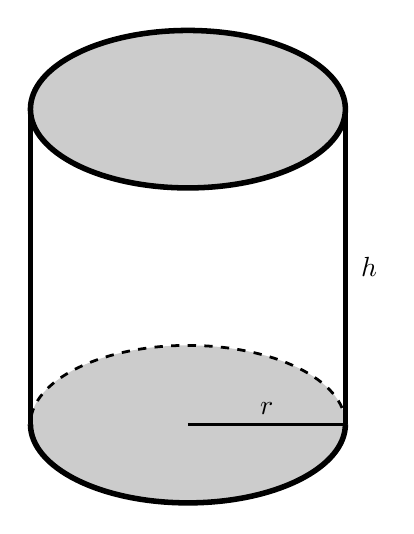
\begin{tikzpicture}
   \onslide<2->
   \begin{scope}[color=black!20]
      \fill (0, 4) circle[x radius=2, y radius=1];
      \fill (0, 0) circle[x radius=2, y radius=1];
   \end{scope}

   \draw[line width=1pt, dashed] (2, 0) arc[start angle=0, delta angle=180, x radius=2, y radius= 1];
\onslide 
   \begin{scope}[line width=2pt]
   \draw (0, 4) circle[x radius=2, y radius=1];
   \draw (2, 0) arc[start angle=0, delta angle=-180, x radius=2, y radius= 1];
   \draw (2 , 0)--(2 , 4);
   \draw (-2 , 0)--(-2 , 4);
   \end{scope}
\onslide<3->
   \node at (2.3,2) {$h$};
   \draw [line width=1pt](0, 0)--(2,0);
   \node at (1, 0.2) {$r$};
\end{tikzpicture}
\end{frame}
% ===================================================================

\end{document}
